\part{Towards Highly Miniaturized LED Power Systems }
\label{ch:twrd_HMLED}

\chapter{The new coming LED based lighting industry}

The appearance of light in the beginnings of the 19th century and the posterior commercialization was clearly a remarkable fact of the past history. The light bulbs contributed in two major facts that impacted peoples life . First, they enabled to have clear, reliable and safe source of light at home, extending our activity hours longer than the natural sun light. As a matter of fact we can not live without the use of artificial light.   Second, the necessity of electric power helped to develop the first electric power distribution systems. Actually, that fact can be still evidenced since people, generally our grand parents, often use the word \emph{light} when they actually are refereing electricity.

\begin{figure}[!h]
\centering
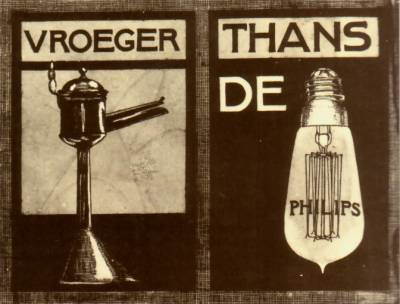
\includegraphics{./0_intro/img/1900-philips3.jpg}
\label{fig:incandescent_light_blub}
\caption{Early incandescent light bulb}
\end{figure}


From the first incandescent light bulb, the lighting industry has not had any big disruptive change to our perception of lighting till the last decade with the apparition of the LED lamps. Besides as many of us thing, it has been done a large effort to improve the efficiency of the light sources while keeping a the quality of the light as good as the incandescent light bulb. Being the florescent lamps one of the biggest contributions during the past century, beginning  to be commercialized around 1930. Later becoming a disruptive change in the lighting market with the introduction the low consumption lamps where Philips was one of the first player launching to the market the first screw-in fluorescent lamp. Although the prices of these lamps has been dropping to become commercially attractive for the costumers, their poorer color rendering factor and the longer setting time compared to the incandescent lamps prevented this lamps to be one-to-one replacement. Therefore the lighting industry has been keep without not too much attention till the introduction the LED based lamps.

\vspace{5mm} %5mm vertical space

\begin{figure}[!h]
\centering
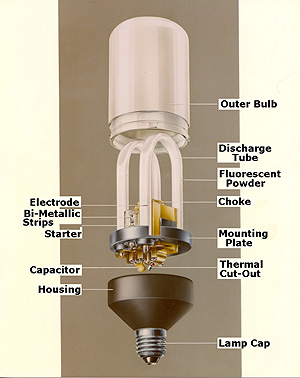
\includegraphics{./0_intro/img/phil1b.jpg}
\label{fig:philips_sl}
\caption{Components of the Philips SL compact fluorescent lamp. }
\end{figure}

The discovery of the high-efficiency blue LED ~\cite{94Nakamura} by Shuji Nakamura in 1994 enabled the quick development of the fist efficient withe LED. These early high power LEDs demonstrated that Solid State Lighting (SSL) devices  where a suitable technology for illumination. The relevance of Nakamura's work has been recognized last year being him awarded with the 2014 Nobel prize in physics. Looking farther we can also confirm the relevance of his invention since the apparition of the LED lamps, lighting is impacting again in our everyday life by changing our traditional concept of luminaries and lighting possibilities.

\begin{figure}[!h]
\centering
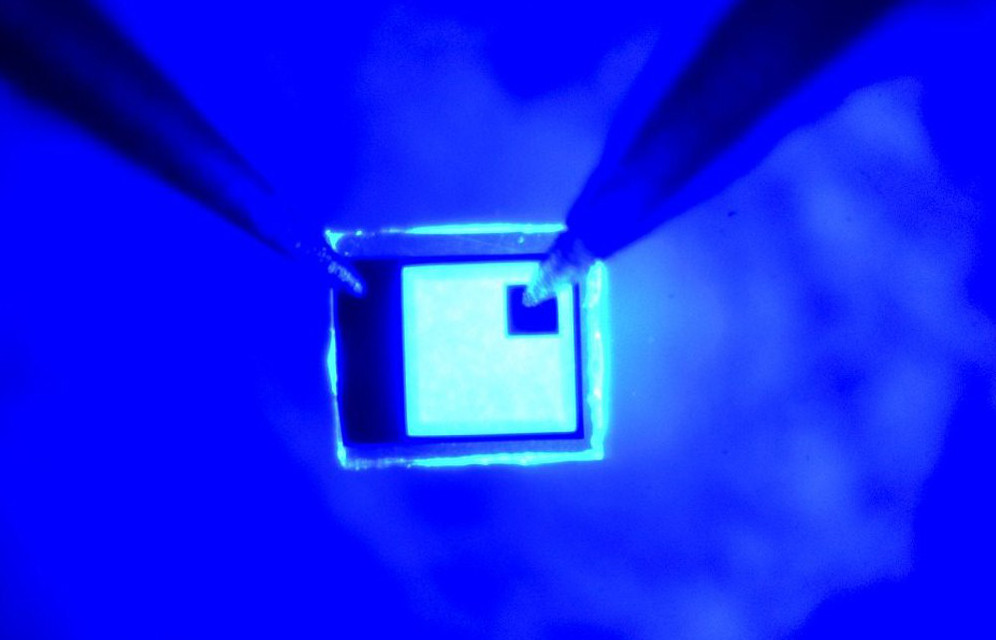
\includegraphics{./0_intro/img/10-7-14-nobel-prize-blue-led.jpg}
\label{fig:blue_LED}
\caption{Picture of a blue LED researched by Shuij Nakamura.}
\caption*{Source: \url{http://www.newsweek.com/how-blue-led-changed-world-and-won-nobel-prize-275977} }
\end{figure}

LED based lamps triggered  a frenetic rush in the lighting industry to bring that technology to the end consumers. Actually the large number of advantages of LED based lighting, or also known as Solid State Lighting (SSL), are so relevant that in the close future will replace any of the present lighting technology, that movement has been already named as the \emph{LEDification}. The principal advantages of SSL are:
\begin{description}
  \item [Efficiency] The light generation inside an LED is produced by the direct mechanism of hold-electron recombination, the supplied energy is a better use of the energy compared to the incandescent lamps. The power consumption can be up to an order of magnitude lower of an incandescent light.

  \item [Size] LEDs are tiny and flat devices, which can be considered as 2-D elements and do not need any vacuum chamber to work. They are much more flexible devices to assembly, and can easily replace the old glass made bulb design.

  \item [Color] LED light has a very narrow light spectrum, that can be used to produce directly colored light. Colored lights are becoming more popular in domestic homes becoming a piece of decoration or mood tweaking device.

  \item [Dynamics] Compared to any of the traditional sources of light LEDs have no dynamics, actually they have but it's very fast and not appreciable to the human eye. Therefore they do not have any setting time when turned on, which is not the case of CFL. The fast dynamics allows to modulate the light and transmit data without disturbing the human beings.

  \item [Lifetime] Solid State devices do not wear off, there fore they can be considered to have an infinite lifetime. In practice LEDs make use of organic phosphores, thus the light quality derates with the use, but the life expectancy of the LED is rated from 20.000 - 100.000 hours, multiplying 20 to 100 times longer that the classical light bulbs.
\end{description}

\vspace{5mm} %5mm vertical space

Bring the LED based lamps to the market is still a big challenge. Despite of the large number of advantages, the end consumers are still very reluctant to change generally due to the elevated costs of the new lamps, currently ranging between \$20 - \$40 for a 100W substitute compared to less than \$3 of an incandescent light. Also another issue that prevents consumers to change to the new technology is a poor light color consistency, light flickering and light dimming incompatibilities, that become really evident in low budget products.

\begin{figure}[!h]
\centering
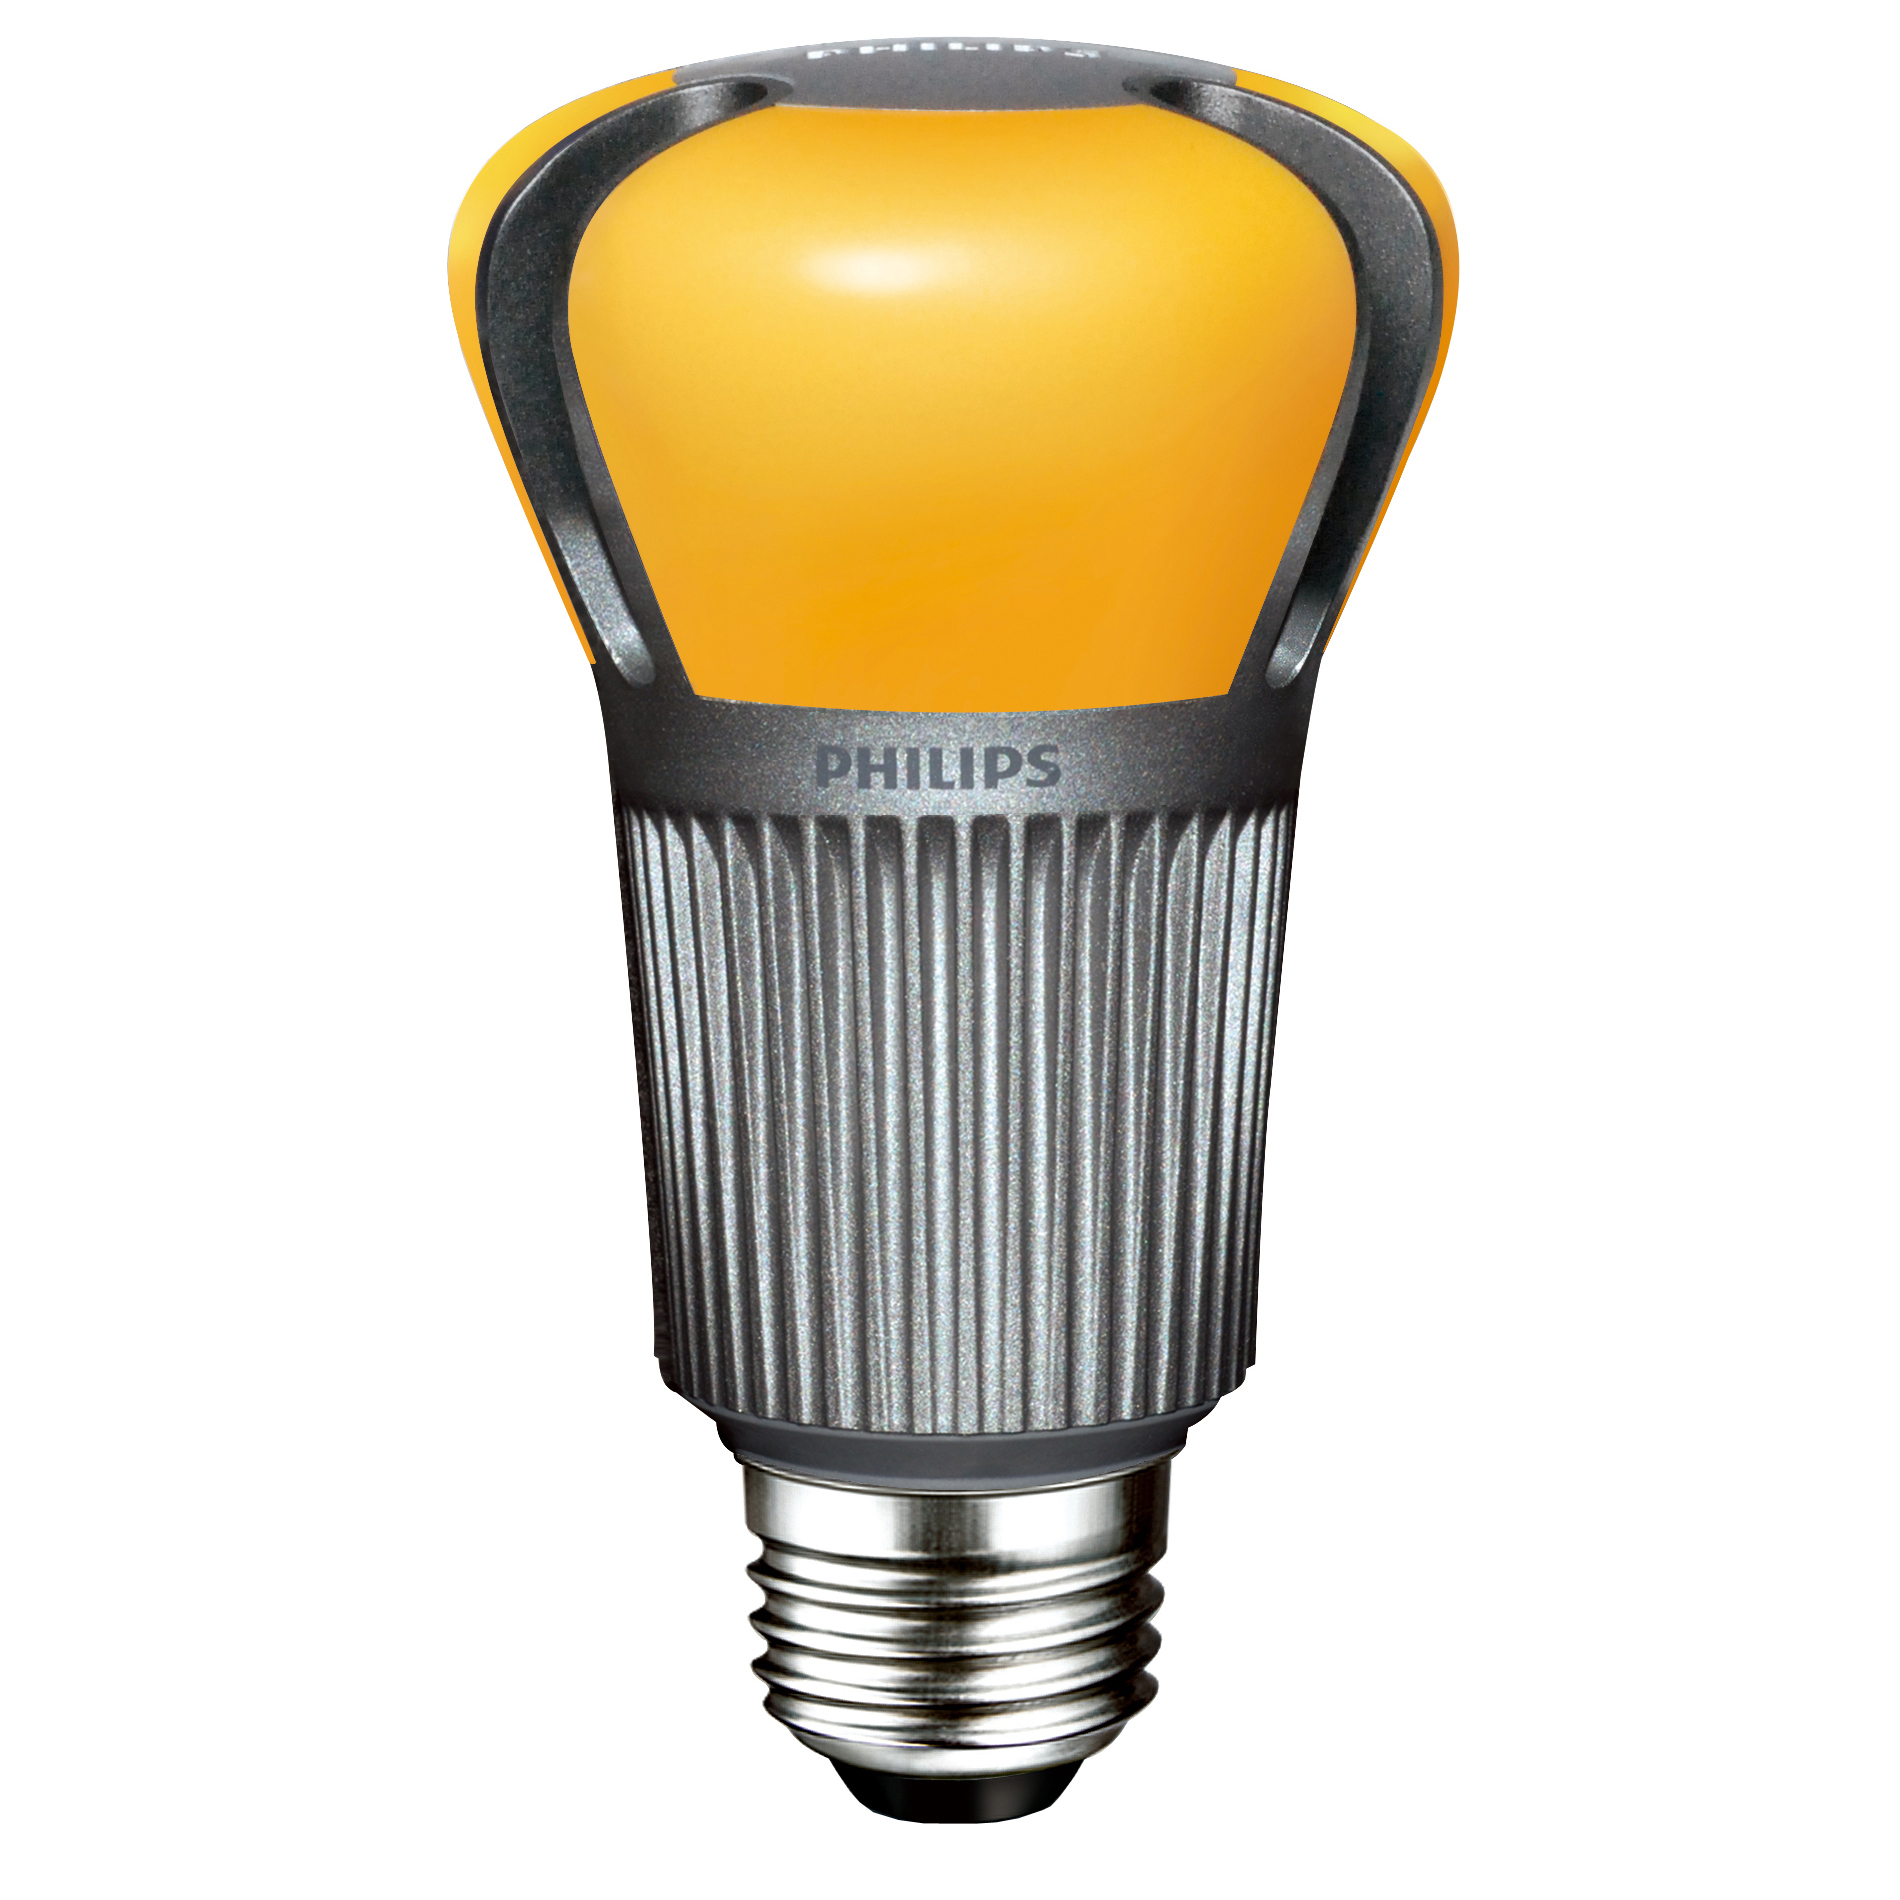
\includegraphics[width=4cm]{./0_intro/img/enduraled-12w.jpg}
\label{fig:l_prize}
\caption{900 lumens LED light bulb.}
\end{figure}

Two factors can be identified to make more favorable the adoption of the SSL as the preferred lighting solution by the consumers. In the one hand, reducing the end product price; and in the other hand, bringing more value to the traditional light sources. Actually LED light bulbs already bring more value compared to the old light bulbs being much more efficient, almost one order of magnitude lower in power consumption, and a longer lifetime, easily twenty times more operating hours. However these factors are not yet a valuable argument for the consumers. With the current trend of the \emph{internet-of-things} remote control, color tuning, light level dimming and integration to with future smart houses are probably some value propositions that people will need and SSL can easily provide. In a second level, I assume that the luminaries designs will change with a more favorable designs that take advantage of the low profiles of the LEDs.

 \begin{figure}[!h]
\centering
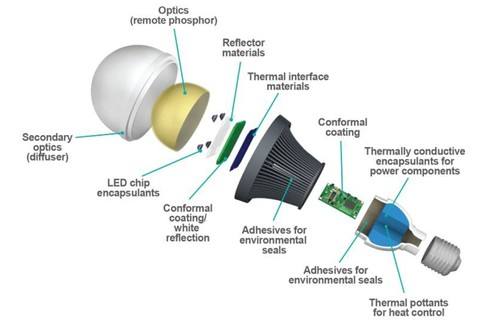
\includegraphics[width=8cm]{./0_intro/img/exploded_bulb_2.jpg}
\caption{Exploded vision of an LED light bulb.}
\label{fig:exploded_bulb}
\end{figure}

It is essential to describe the different elements in a LED light bulb in order to understand the challenges in its development and  design. A LED light bulb is composed by the six main elements described below and shown in  the Fig. ~\ref{fig:exploded_bulb}.

\begin{description}
  \item[LED] A two-lead semiconductor device that produced light when a current flows through it. The name comes from its acronym \emph{Light-Emitting Diode}. The light is produced by electroluminescence when an electron recombines with an electron-hole releasing energy in form of photons. The color of the light is determined by the energy band gap of the semiconductor.

   LED cost is very cheap and there is a broad assortment in colors, power and applications. The selection of the LED will determine: light color, voltage and current of the load, efficiency and necessary optics.

  \item[Optics] The optical device that helps to collimate, mix and distribute the light in the space in a desired way, normally uniformly for a determined projection area.

  \item[Driver] Electronic circuit placed between the input source and the load, the LEDs, that transforms the input electrical power to the requirements of the load. Since almost all the power distribution systems and storage devices are voltage sources and LEDs are current supplied loads, an LED driver is considered as current-to-voltage (V-I) power supply.

      The driver controls the current thought the load, hence the light output. Therefore it can be considered as the active part of the system where the control of the lamp relies. It is the most expensive and takes the largest volume of the lamp, and also one of the most or even the most important element in the entire system.

  \item[Heat sink] Mechanical element that acts as a passive heat exchanger and cools hot elements within the lamps system by dissipating the heat into the surrounding medium. The energy that is not converted to light becomes heat and must be extracted from the lamp, the main heat contributors elements are the LEDs and some components of the driver.

      The costs of the heat sink is also a relevant part in the total cost of the lamp.

  \item[Body assembly] Mechanical element that hold all the different subsystems in one single device. In many cases the heat sink does this functionality.

  \item[Connector] Mechanical element that provides connection with the energy source. The most popular one is the Edison connector present in all screw-in lamps. There are many other popular ones such as GU10, MR16, MR11 coming from the halogen multifaceted reflector bulbs or the 2-pin connector of the fluorescent tubes.

      In many cases, the standardized connectors suppose a restriction for the mechanical design of the lamp. Their old-fashioned design is not optimal for the new lamps.


\end{description}

\vspace{5mm} %5mm vertical space

The chart shown in Fig.\ref{fig:cost_breakdown} makes evident that the driver is the most expensive part of the system. As it was previously mentioned, the driver is the key component in the functionality of the LED lamp, since it controls the light output and at the same time determines the efficiency of the system. Therefore, the LED driver has become on of the hot topics of research within the power electronics field. Besides the necessity of fulfilling the operational requirements, such as high efficacy an proper power quality, two main issues have trigger research around the driver circuit: The costs and the volume.
\begin{figure}[!h]
\centering
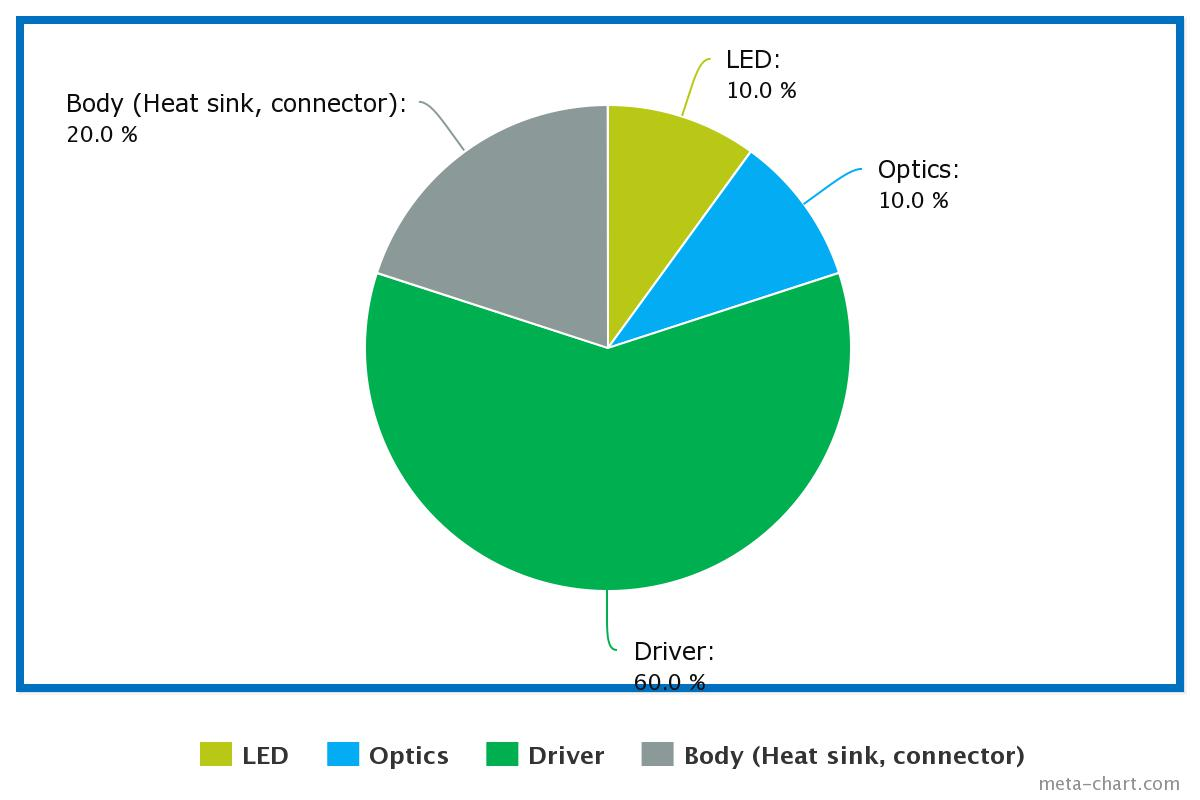
\includegraphics[width=8cm]{./0_intro/img/piechar_costs.jpeg}
\caption{LED lamp cost breakdown by subsystems.}
\label{fig:cost_breakdown}
\end{figure}

\vspace{5mm} %5mm vertical space

The cost of the driver is one of the biggest problems that SSL industry has been dealing after the power LEDs become a commodity components. Actually, this piece of electronics was not present in the incandescent light bulbs, thus its elevated cost arose as an inconvenient and difficult to justify in the new light bulbs. Philips Research has devoted a large effort in that field, being indeed the main focus of research regarding the LED drivers.


Reducing the costs of the lamps has been the strategy taken for the first wave in the \emph{LEDification} process where retrofitting\footnote{Adding the new LED technology to the older light bulb systems. In that way the end user can directly replace an incandescent lamp or a florescent tub by an LED one without needing to make any change in the current installation.} the old lamps is chosen as the way to target the end costumer. In on the one hand, fruitful results came form that research with new innovative solutions at very low costs that could be packed in almost all the light bulb shapes currently commercially available. But in the other hand, these new drivers had the incontinent of using very old components that at the same time restricted reduction of the circuit volume and made more complex the addition of extra control functionalities while keeping the initial low costs.

\begin{figure}[!h]
\centering
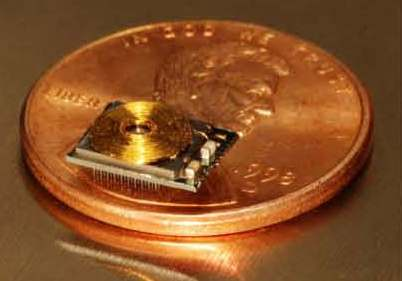
\includegraphics[width=8cm]{./0_intro/img/FSolzbacher01.jpg}
\caption{Power System in a Package die. The circuit implements a buck converter.}
\label{fig:psoc_example}
\end{figure}

\vspace{5mm} %5mm vertical space

The second line of research has focus on reducing the volume of the driver circuit. That research topic arose when comparing the the volume of the LEDs and the driver, it is evidenced a mismatch between the two volume of the components, becoming in many cases the driver circuit the dominant element of the entire lamp. Such mechanical constrain supposes an obstacle to take the full advantage of the low form-facto of the LED in the future luminaries, where LED will not be assembled using the old fashioned cases. Therefore, that research has a much longer term vision for targeting the second of third generation of lights in the \emph{LEDification} process.

The drive to reduce the volume of the drivers led to focus the research from the perspective of the integrated power supplies, where the power converter can be partially or fully integrated in a single package. There are two approaches of integrated power converters: \emph{Power System on Chip} (PSoC) or  \emph{Power System in Package} (PSiP). The first integrate all required power components, active and passive, in a single die. The second assemble all the components within the same package, keeping the appearance of an unique \emph{Integrated Circuit} (IC), see Fig.\ref{fig:psoc_example}. The advantages of having an integrated power management unit align with the necessities of the LED drivers, therefore trend of the drivers will be going towards having \emph{Power LED Drivers in Package} (PLDiP).

Besides the size reduction that an integrated driver would suppose, an integrated approach would also bring other benefits in terms of control and connectivity. Since such a solution would require a the design of a dedicated \emph{application-specific integrated circuit} (ASIC), the power management unit and driver control unit can be integrated together, providing the necessary intelligence for light control and the connectivity optimized for the requirements of the coming connected lighting industry. The \emph{Philips} \emph{HUE} lamp is a clear example of the requirements of the so called \emph{smart drivers}. That lamp provides a full light color gamut color control through a mobile and web application or through a remote control. The internal driver has four light channels red, green, orange and additional amber and at the same time provides wireless connectivity through ZigBee, being the electronic board populated with discrete power drivers and few micro-controller units. A solution that integrates all the functions in a single IC, or few ICs (one per channel), will definitely reduce packaging and assembling costs and still providing the same functionalities. And at the same time, the expected market size for LED lighting to justify a dedicated ASIC design for the light bulbs and indeed has been the motivation of this thesis. Therefore goal of this work was to explore and identify new architectures that are suitable for integration and at the same time can perform as an efficient LED driver.


\section{Why a LED needs a driver?}

As shown in Fig. \ref{fig:led_I-V} a LED has a very abrupt V-I curve. For voltages below the \emph{forward voltage}, $V_{f}$, there is no current flow and the LED behaves as an open circuit. For voltages above $V_{f}$ the curve becomes very steep and the current increases dramatically with respect to the voltages, thus the LED behaves as short circuit. The driver bias the LED to a specific point, $P$ in Fig. \ref{fig:led_I-V}, providing the desired output light. The colour and flux (light intensity) will vary depending of the bias point.  Since the majority of  available  energy sources are  voltage sources, and LED requires a circuit that limits the current that flows through it, that circuit is the LED driver.

\begin{figure}[!h]
\centering
\begin{tikzpicture}[domain=0:5]
    \draw [->] (0,0) -- (4.5,0) node[anchor=west]{$V$};
    \draw [->] (0,0) -- (0,4.5) node[anchor=east]{$I$};

    %Mark Vth
    \draw (2,2pt) -- (2,-5pt) node[anchor=north] {$V_{f}$};

    %Draw ideal plot
    \draw[thick] (0,0) -- (2,0) -- (4,4);

    %Draw bias points
    \draw[dashed] (3,2) -- (3,-0);
    \draw (3,2pt) -- (3,-5pt) node[anchor=north]  {$V_{bias}$};

    \draw[dashed] (3,2) -- (-0,2);
    \draw (2pt,2) -- (-5pt,2) node[anchor=east]  {$I_{bias}$};
    \filldraw (3,2) circle(2pt) node[anchor=west] {$P$};

  

\end{tikzpicture}
\caption {}
\label{fig:led_I-V}
\end{figure}

At the first glance, keeping a constant bias current, $I_bias$, through the LED does not seems to be challenging. However LED V-I characteristic is not static, in practice LEDs has different source of deviations and drivers have to deal with them in order to keep delivering the desired light output. First, $V_f$ has a negative dependence with the temperature, drooping its values as the PN junction temperature increases. Second, the LED has an aging factor derating its light output over time, which has to be adjusted by changing the bias point. And last but not least, during production LEDs will vary in colour, flux and forward voltage; even for products from the same batch. The manufacturer reduced the dispersion between devices by binning \footnote{Quality control performed at LED production line, where each LED is individual tested and sorted in groups (bins) that have the same electrical and lighting characteristics.}, but still after binning it can be deviations from up to $10\%$ in $V_f$ for the same part number.

Up to date, there are three families of LED drivers:

\begin{description}
  \item[Linear Drivers] place a shunt element between the source and the LED. The shunt element limits the current in the LED providing the necessary voltage droop between the source and the load. The excess of voltage between the source and the load is dissipated in the shunt element, literally burned in form of heat; therefore this drivers become very inefficient if the LED voltage is not close to the source. Moreover this drivers can only provide step-down conversion, thus they cannot work when the load voltage is higher than the input supply.

      \begin{figure}[!h]
        \centering
        \ctikzset { bipoles/length=1cm}
        \begin{circuitikz} [american,scale=0.65]
        \draw
        (5,0) to[short]
        (0,0) to[V = $v_{src}$]
        (0,3) to[generic=${Shunt}$]
        (5,3);
        \draw
        (5,0) to[leD*,mirror,v>=$v_{o}$,i<=$i_o$] (5,3); 
        
        \begin{scope}[xshift = 8cm, yshift=0cm]
            \draw[->] (0,0) -- (4,0) node[anchor=north] {$  m $};
            \draw[->] (0,0) -- (0,3) node[anchor=west] {$\eta $};
            
            %Ticks X 
            \draw (3,2pt) -- (3,-5pt) node[anchor=north] {$1$};
            \draw (1.5,2pt) -- (1.5,-5pt) node[anchor=north] {$0.7$};
            
            %Ticks Y
            \draw (2pt,2.5) -- (-5pt,2.5) node[anchor=east] {$100\%$};
            \draw (2pt,1.5) -- (-5pt,1.5) node[anchor=east] {$70\%$};
            
            %Markers
            \draw[dotted] (3,2.5) -- (3,0);
            \draw[dotted] (3,2.5) -- (0,2.5);
            \draw[dotted] (1.5,1.5) -- (1.5,0);
            \draw[dotted] (1.5,1.5) -- (0,1.5);
            
            
            \draw[thick] (3,2.5) -- (0,0.5);
            
            
            
        \end{scope}
        
        \end{circuitikz}
        \label{fig:linear_drv}
        \caption{Linear LED driver schematic} 
       \end{figure}
      
   The circuit of the Fig. \ref{fig:linear_drv} shows schematic of a linear driver, the shunt element can be implemented with just a resister of with an active device, the second enables regulation for variations in the source and in the load. Both cases linear drivers are very simple to implement, with very low costs and taking almost no volume, being indeed the perfect solution for integration.
   
   The plotted graph presents the variation of the driver efficiency with respect to the conversion ration $m$. $m$  is the ratio between the input voltage, $v_{src}$,  and the output voltage,$v_o$, being defined as
   \begin{equation}
        m = \frac{v_o}{v_{src}}.
   \end{equation}
   
   The efficiency of the driver is the ratio between the input power and the output power
   \begin{equation}
        \eta = \frac{P_o}{P_i} = \frac{v_o i_o}{v_{src} i_o} = \frac{v_o}{v_{src}},
   \end{equation}
   thus we can see that for this case the efficiency is indeed the conversion ratio
   \begin{equation}
        \eta = m,
   \end{equation} 
   owing to the fact that LED drivers have to be efficient, saying that at worst case 80\% efficiency can be accepted, such drivers could only be suitable where the ration between input voltage and load voltage is 0.8.  
   
   Despite the fact that linear drivers are cheap and easy to integrate, their poor efficiencies and limitations in power conversion palace them in a unfavorable position as a realistic sortition for an integrated solution.  
   
   


  \item[Inductor Based Converters] are \emph{Switched Mode Power Supplies} (SMPS) 
  \item[Switched Capacitors] dfa
\end{description}


\chapter{Different types of Drivers}




%\section{DC-DC Drivers}
%\section{AC-DC Drivers}

\chapter{Switched capacitors for LED drivers}

There are two families within the integrated power supplies, inductor based converters and switched capacitors based converters. Inductor based converters make use of magnetic passive components as energy storage for the power conversion, being the most common converters used for LED drivers for to lighting. These converters easily achieve very large efficiencies while providing excellent current regulation output. However the magnetic devices restricts the integration of these converters. Switched Capacitor Converters (SCC) provide energy conversion using capacitors as a energy storage


